\documentclass[border=3pt,tikz]{standalone}
\usepackage{amsmath}
\usetikzlibrary{arrows}
\usetikzlibrary{positioning}
\usetikzlibrary{calc}
\usetikzlibrary{arrows.meta}
\usetikzlibrary{decorations.pathreplacing}
\begin{document}
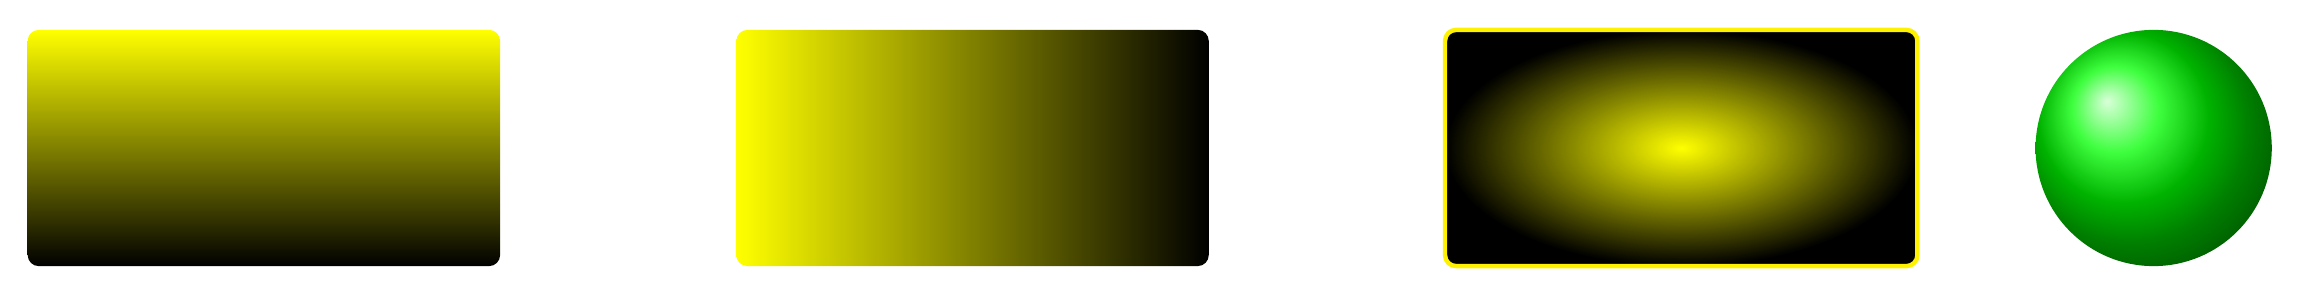
\begin{tikzpicture}[scale = 3, rounded corners,ultra thick]
    \shade[top color=yellow,bottom color=black] (0,0) rectangle +(2,1);
    \shade[left color=yellow,right color=black] (3,0) rectangle +(2,1);
    \shadedraw[inner color=yellow,outer color=black,draw=yellow] (6,0) rectangle +(2,1);
    \shade[ball color=green] (9,.5) circle (.5cm);
  \end{tikzpicture}
\end{document}